В ходе работы также было проведено исследование зависимости показателей качества от частоты кадров видеоизображения. 
Мотивация этого сравнения заключается в том, что при запуске на микрокомпьютере скорость работы заметно ниже, а значит временные промежутки между кадрами больше. 
В следствии этого, объекты на изображении будут перемещаться сильнее между кадрами, что повлияет на качество отслеживания. 
Именно поэтому, для адекватного сравнения алгоритмов между собой, важно пересчитать метрики для разных показателей частоты кадров. 

На рисунках \ref{fig:fps_ByteTrack}-\ref{fig:fps_ImprAssOC} виден результат проведенного сравнения. 
Все показатели медианные для каждого алгоритма. 
Для анализа выбраны детекторы yolov8n и yolov8s, так как только они способны запускаться на микрокомпьютере с частотой кадров больше 10, а так же yolov8x как эталон возможного максимума.
Частоты кадров видеоизображения для сравнения подобраны методом кластеризации k-средних всех полученных результатов частоты работы на микрокомпьютере.

По полученным результатам четко видна общая закономерность почти для всех методов: 
\begin{itemize}
    \item до 5 кадров в секунду идет значительный линейный рост показателей метрик HOTA, MOTA и IDF1;
    \item с 5 до 11 происходит небольшое улучшение;
    \item при частоте выше 11 показатели или выходят на плато, или растут незначительно.
\end{itemize}
Вероятно, это является следствием увеличения шумов с ростом частоты кадров видеоизображения, так как перемещения между кадрами становятся все меньше и меньше, а погрешность детектора в несколько пикселей начинает играть всю большую роль и перевешивает плюсы от меньших перемещений.

\begin{figure}[ht]
    \centering
    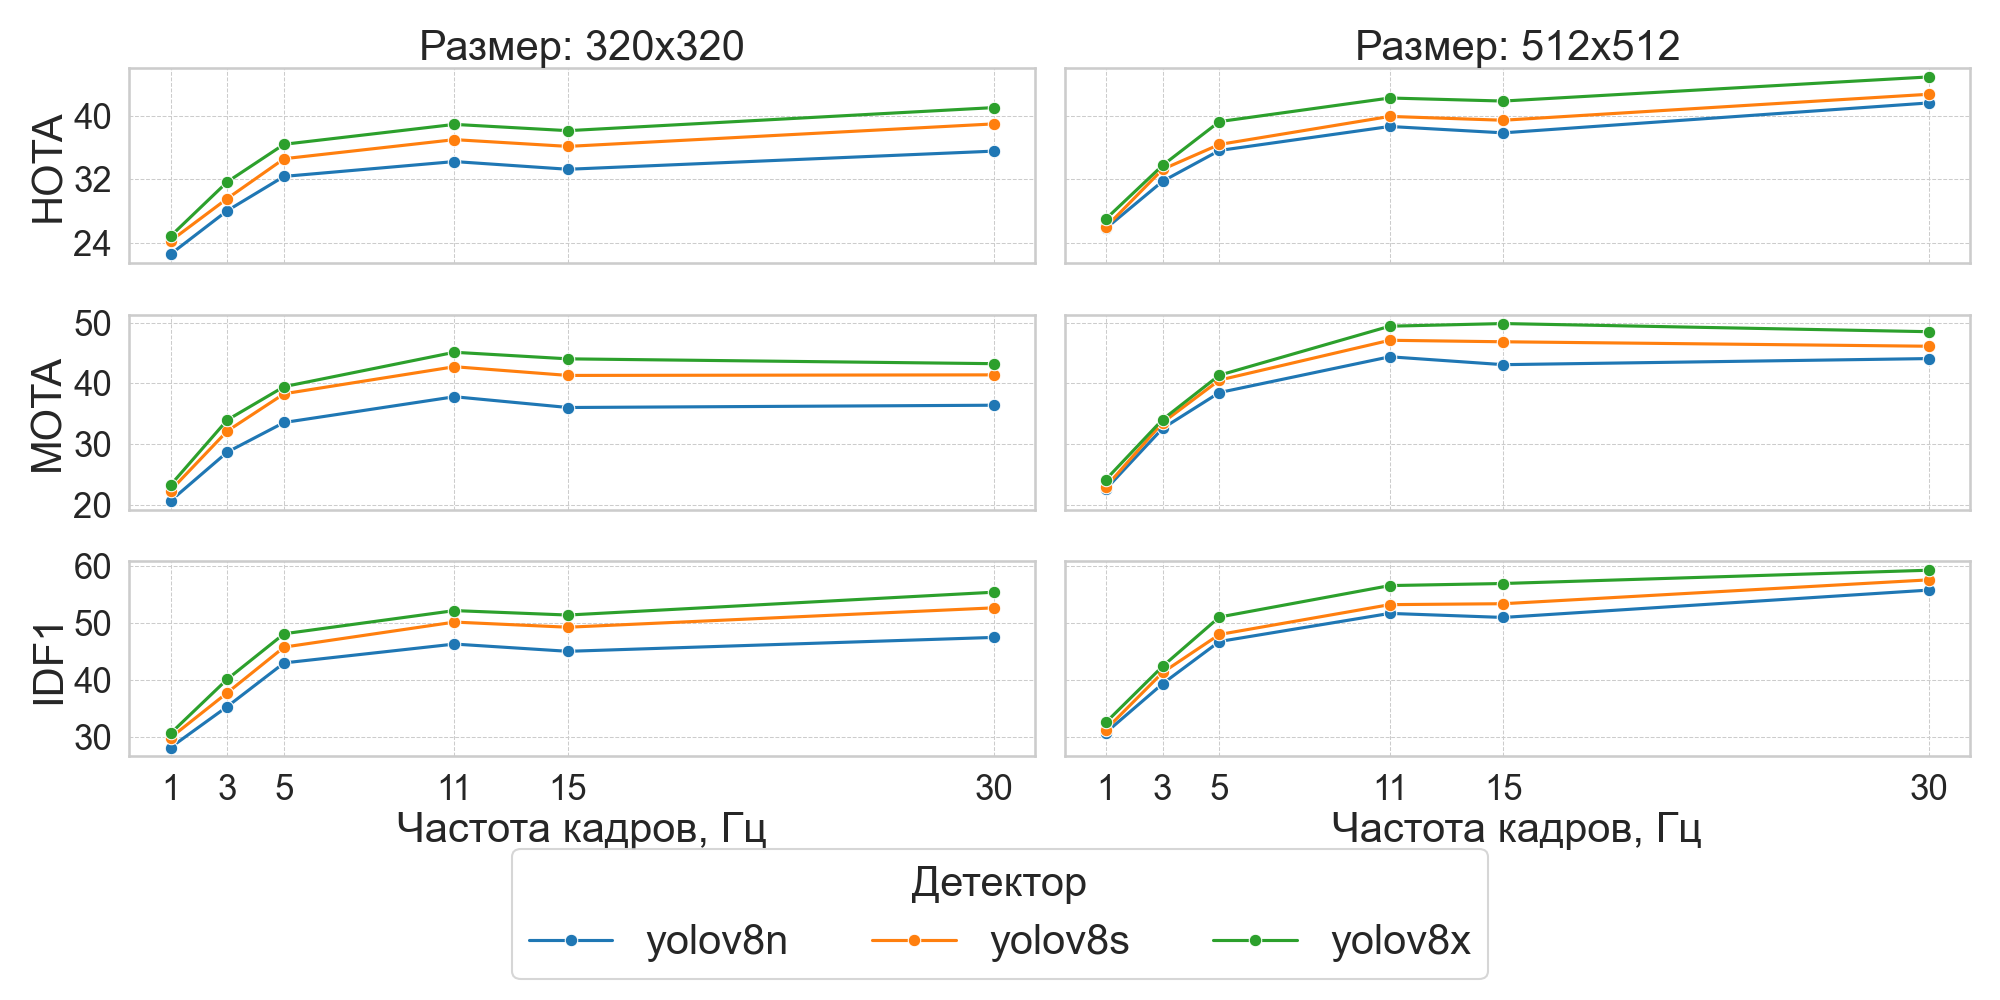
\includegraphics[width=1\textwidth]{plots/fps_vs_metric/ByteTrack.png}
    \caption{График зависимости метрик HOTA, MOTA и IDF1 от частоты кадров видеоизображения для алгоритма ByteTrack}
    \label{fig:fps_ByteTrack}
\end{figure}

\begin{figure}[ht]
    \centering
    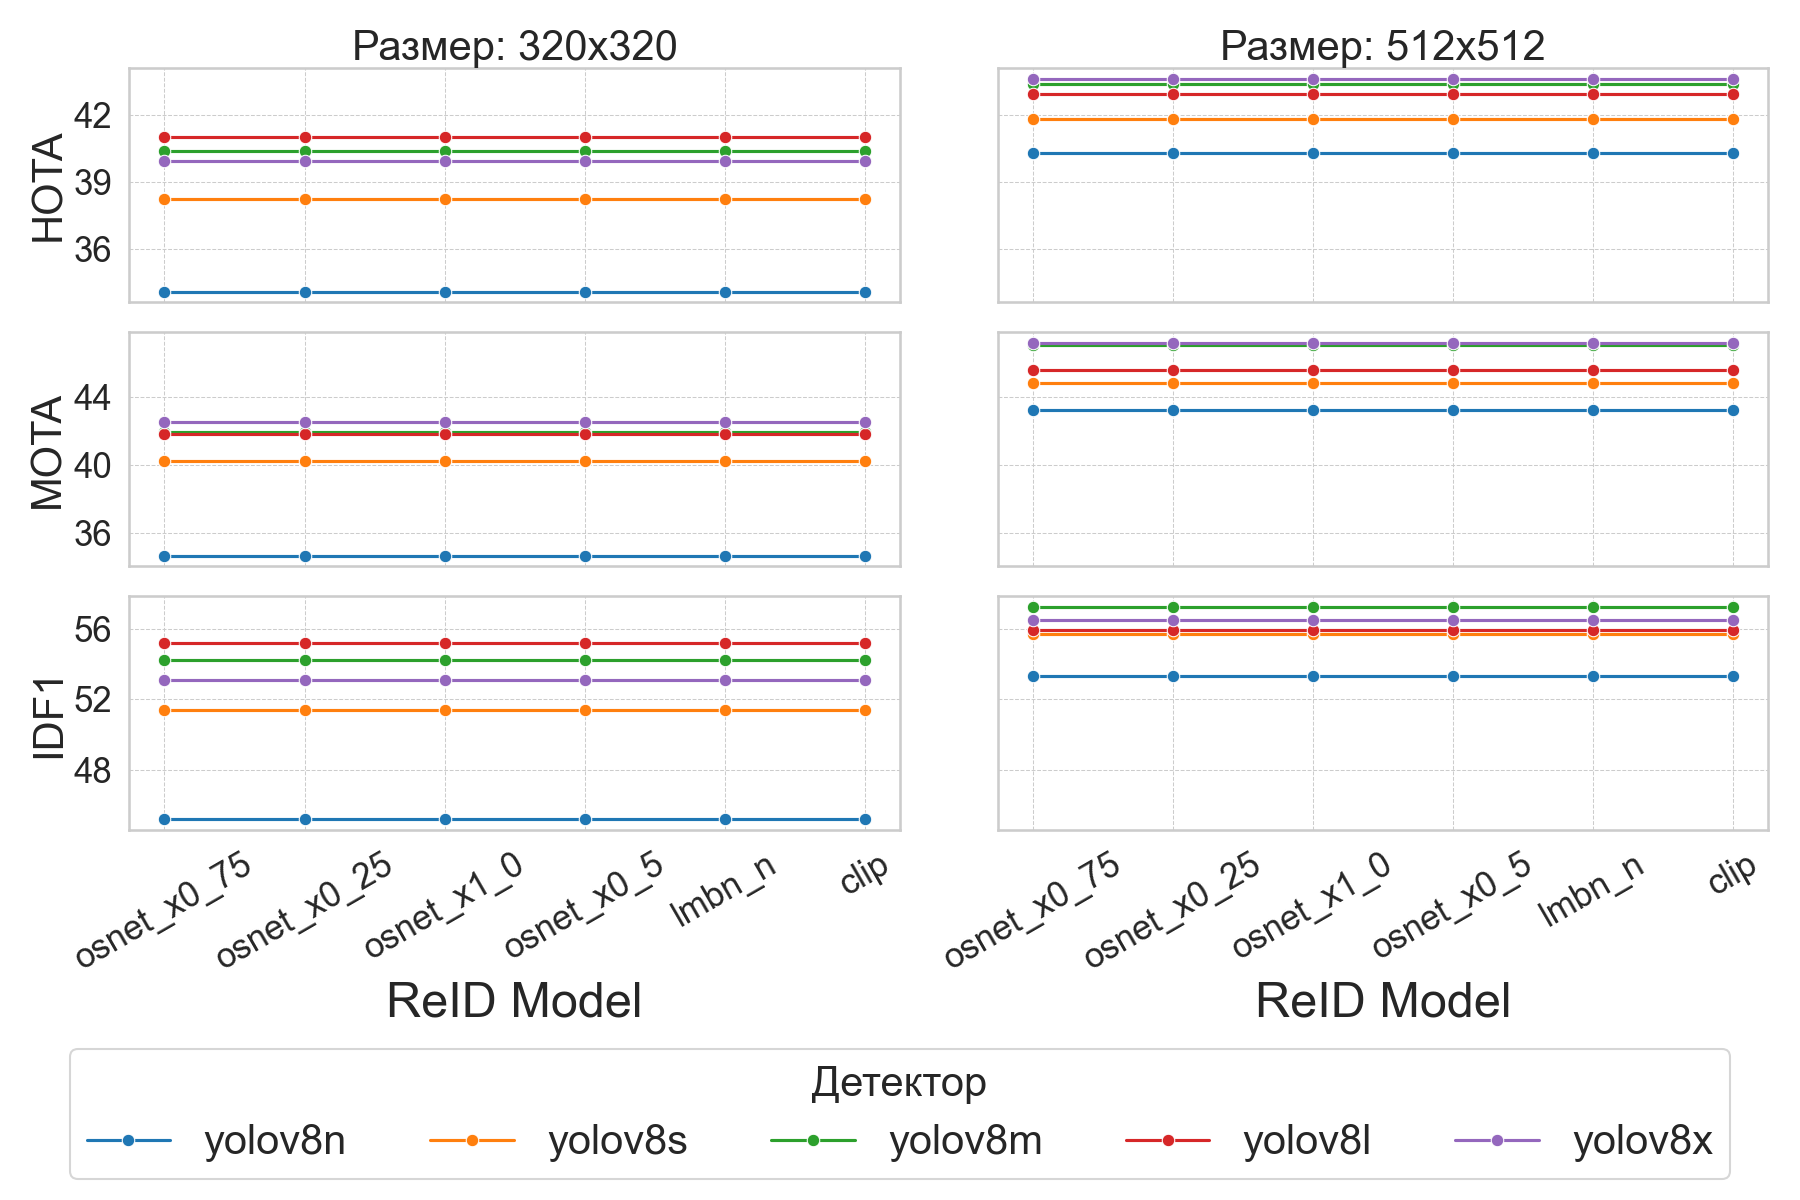
\includegraphics[width=1\textwidth]{plots/fps_vs_metric/OC-SORT.png}
    \caption{График зависимости метрик HOTA, MOTA и IDF1 от частоты кадров видеоизображения для алгоритма OC-SORT}
    \label{fig:fps_OC-SORT}
\end{figure}

\begin{figure}[ht]
    \centering
    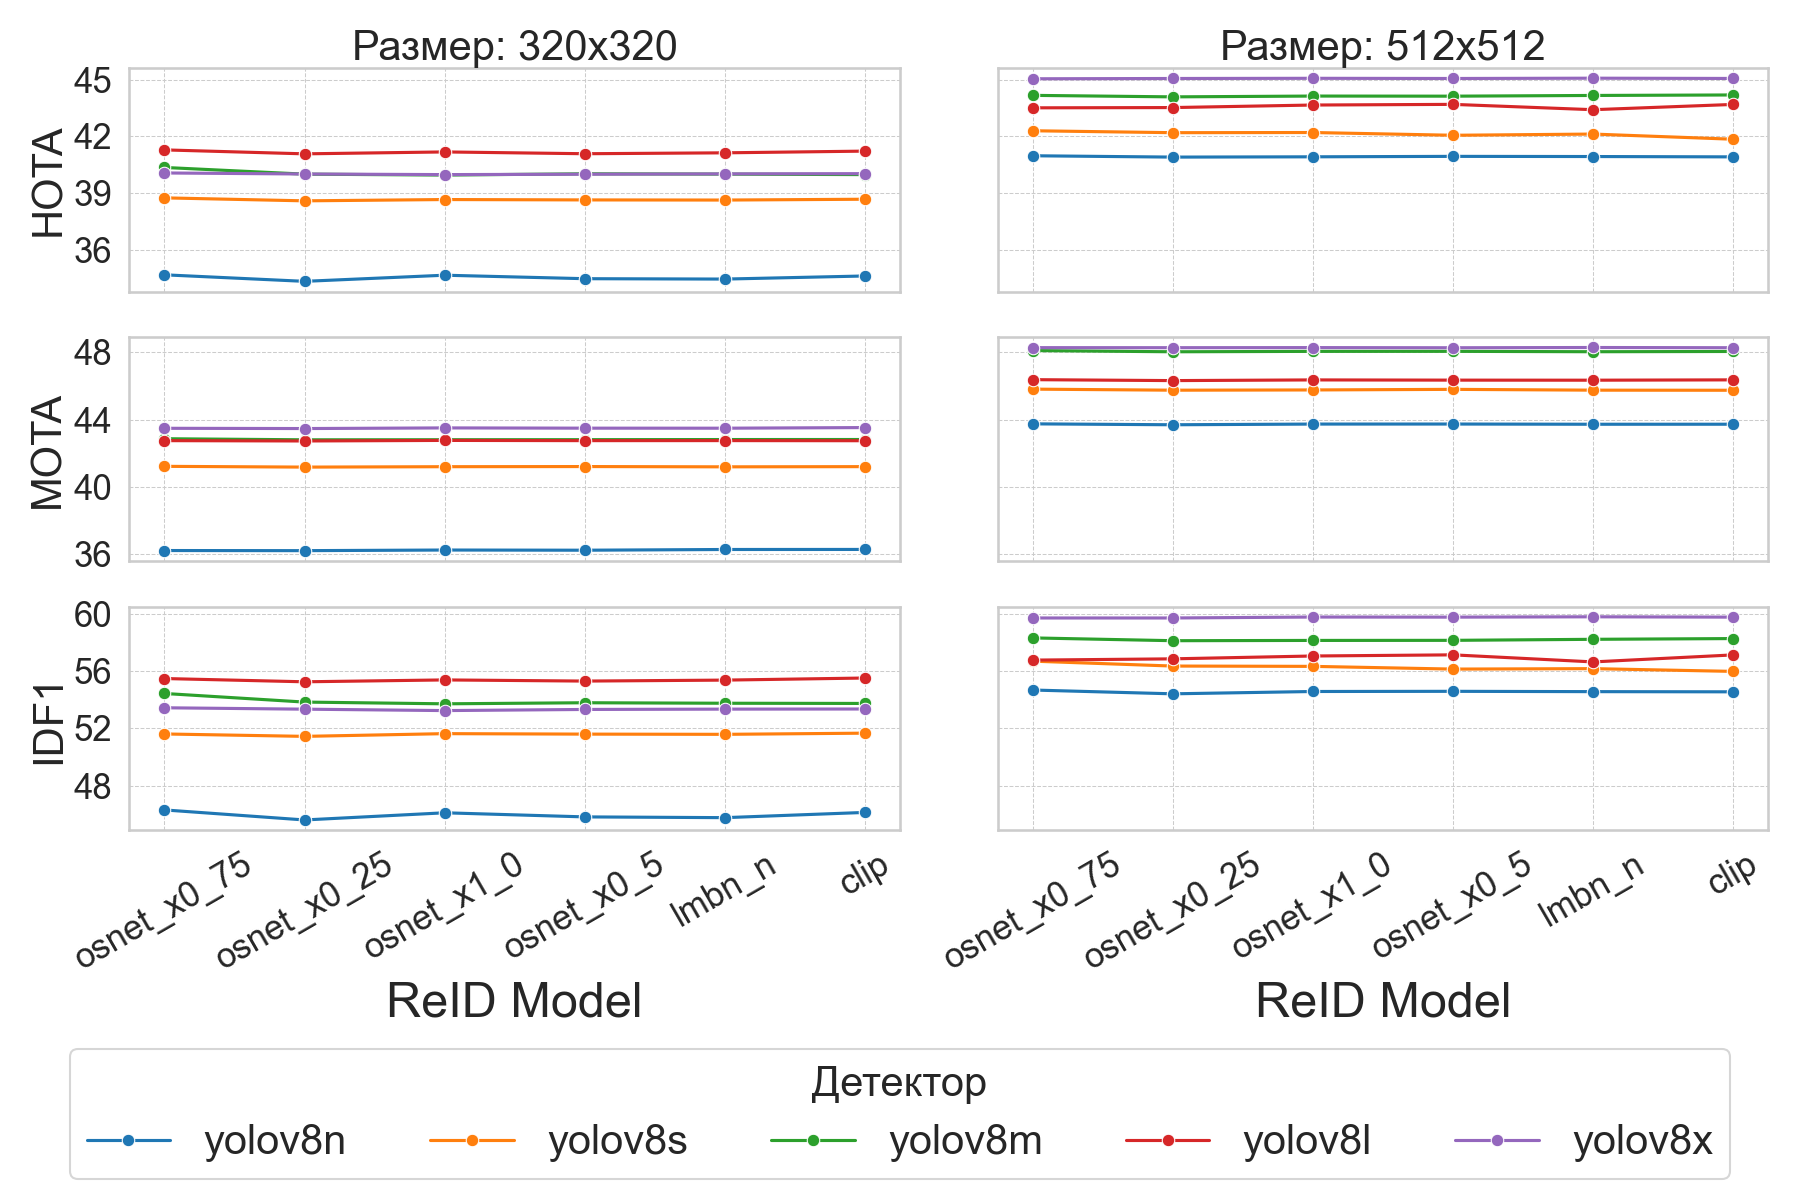
\includegraphics[width=1\textwidth]{plots/fps_vs_metric/Deep OC-SORT.png}
    \caption{График зависимости метрик HOTA, MOTA и IDF1 от частоты кадров видеоизображения для алгоритма Deep OC-SORT}
    \label{fig:fps_Deep OC-SORT}
\end{figure}

\begin{figure}[ht]
    \centering
    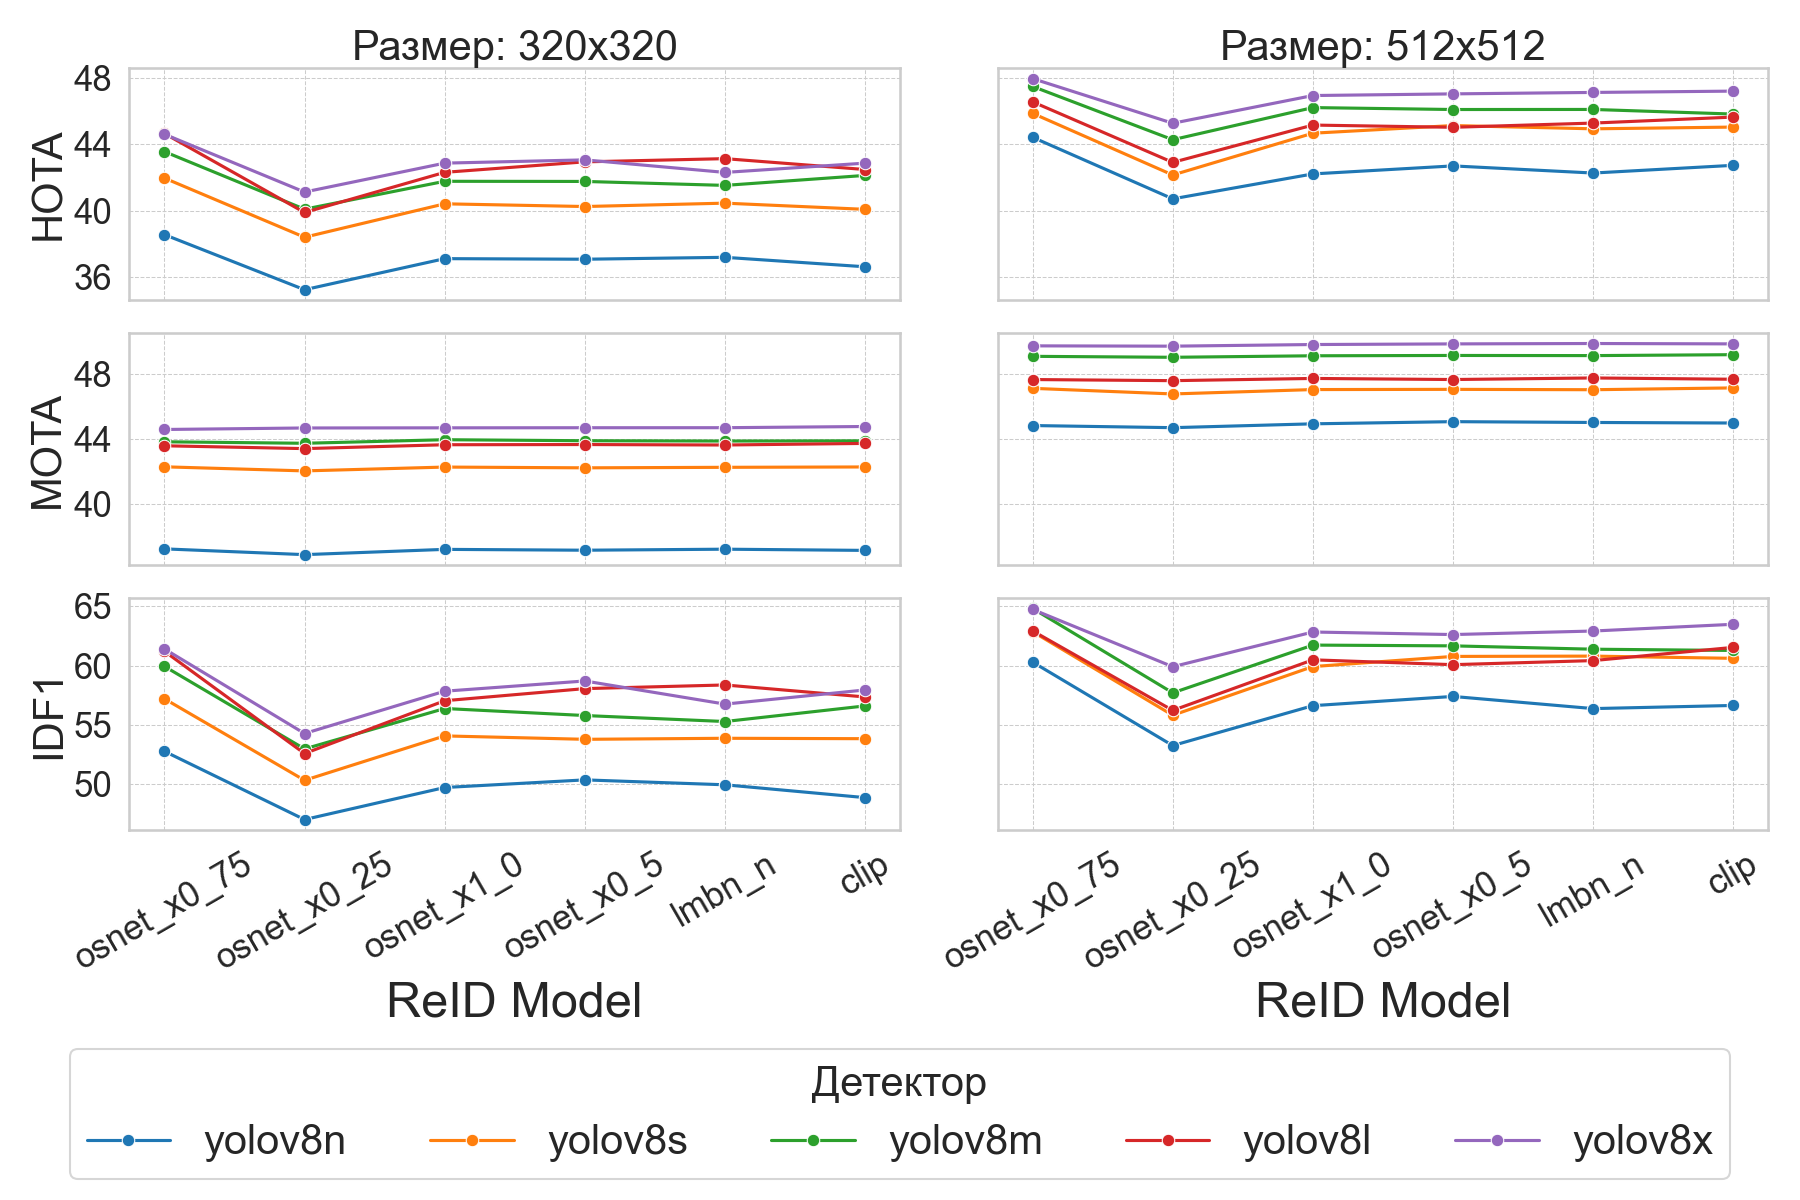
\includegraphics[width=1\textwidth]{plots/fps_vs_metric/StrongSORT.png}
    \caption{График зависимости метрик HOTA, MOTA и IDF1 от частоты кадров видеоизображения для алгоритма StrongSORT}
    \label{fig:fps_StrongSORT}
\end{figure}

\begin{figure}[ht]
    \centering
    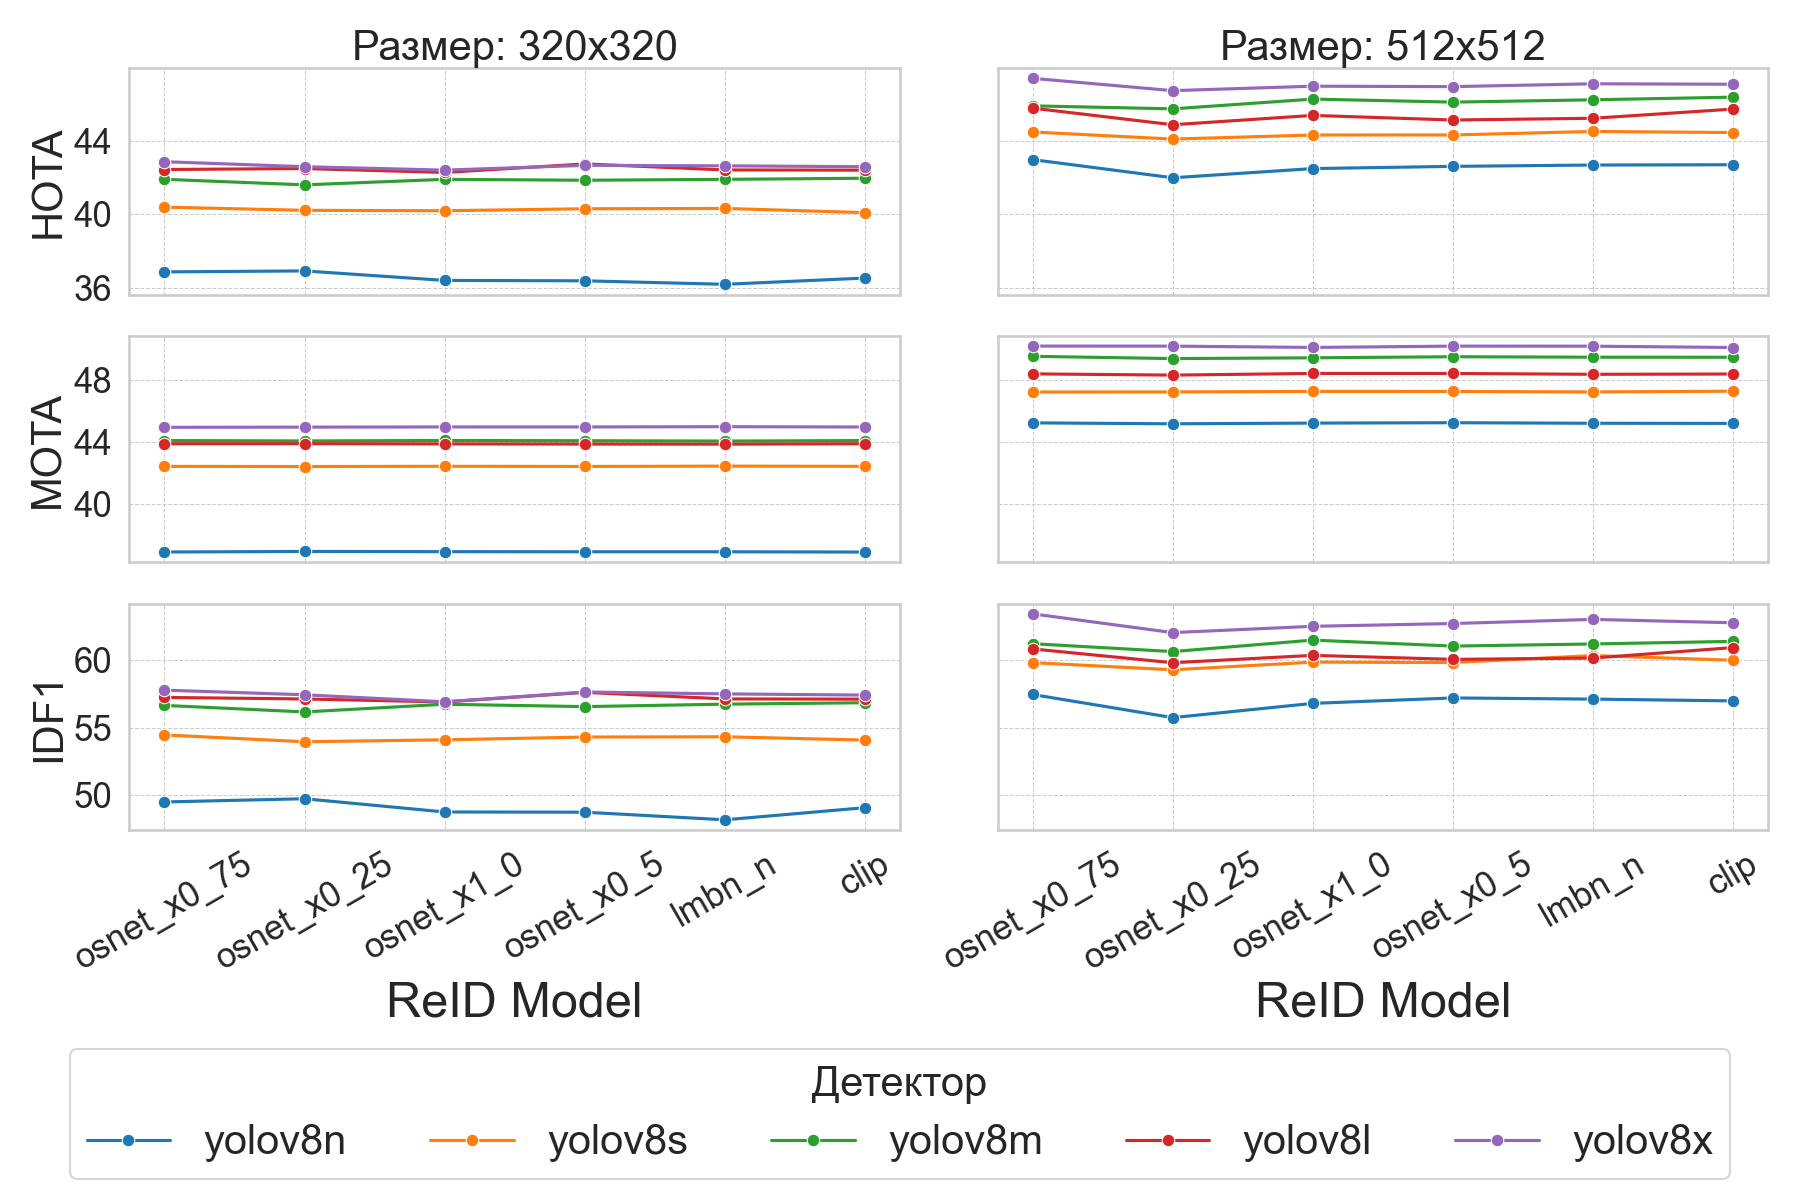
\includegraphics[width=1\textwidth]{plots/fps_vs_metric/BoT-SORT.png}
    \caption{График зависимости метрик HOTA, MOTA и IDF1 от частоты кадров видеоизображения для алгоритма BoT-SORT}
    \label{fig:fps_BoT-SORT}
\end{figure}

\begin{figure}[ht]
    \centering
    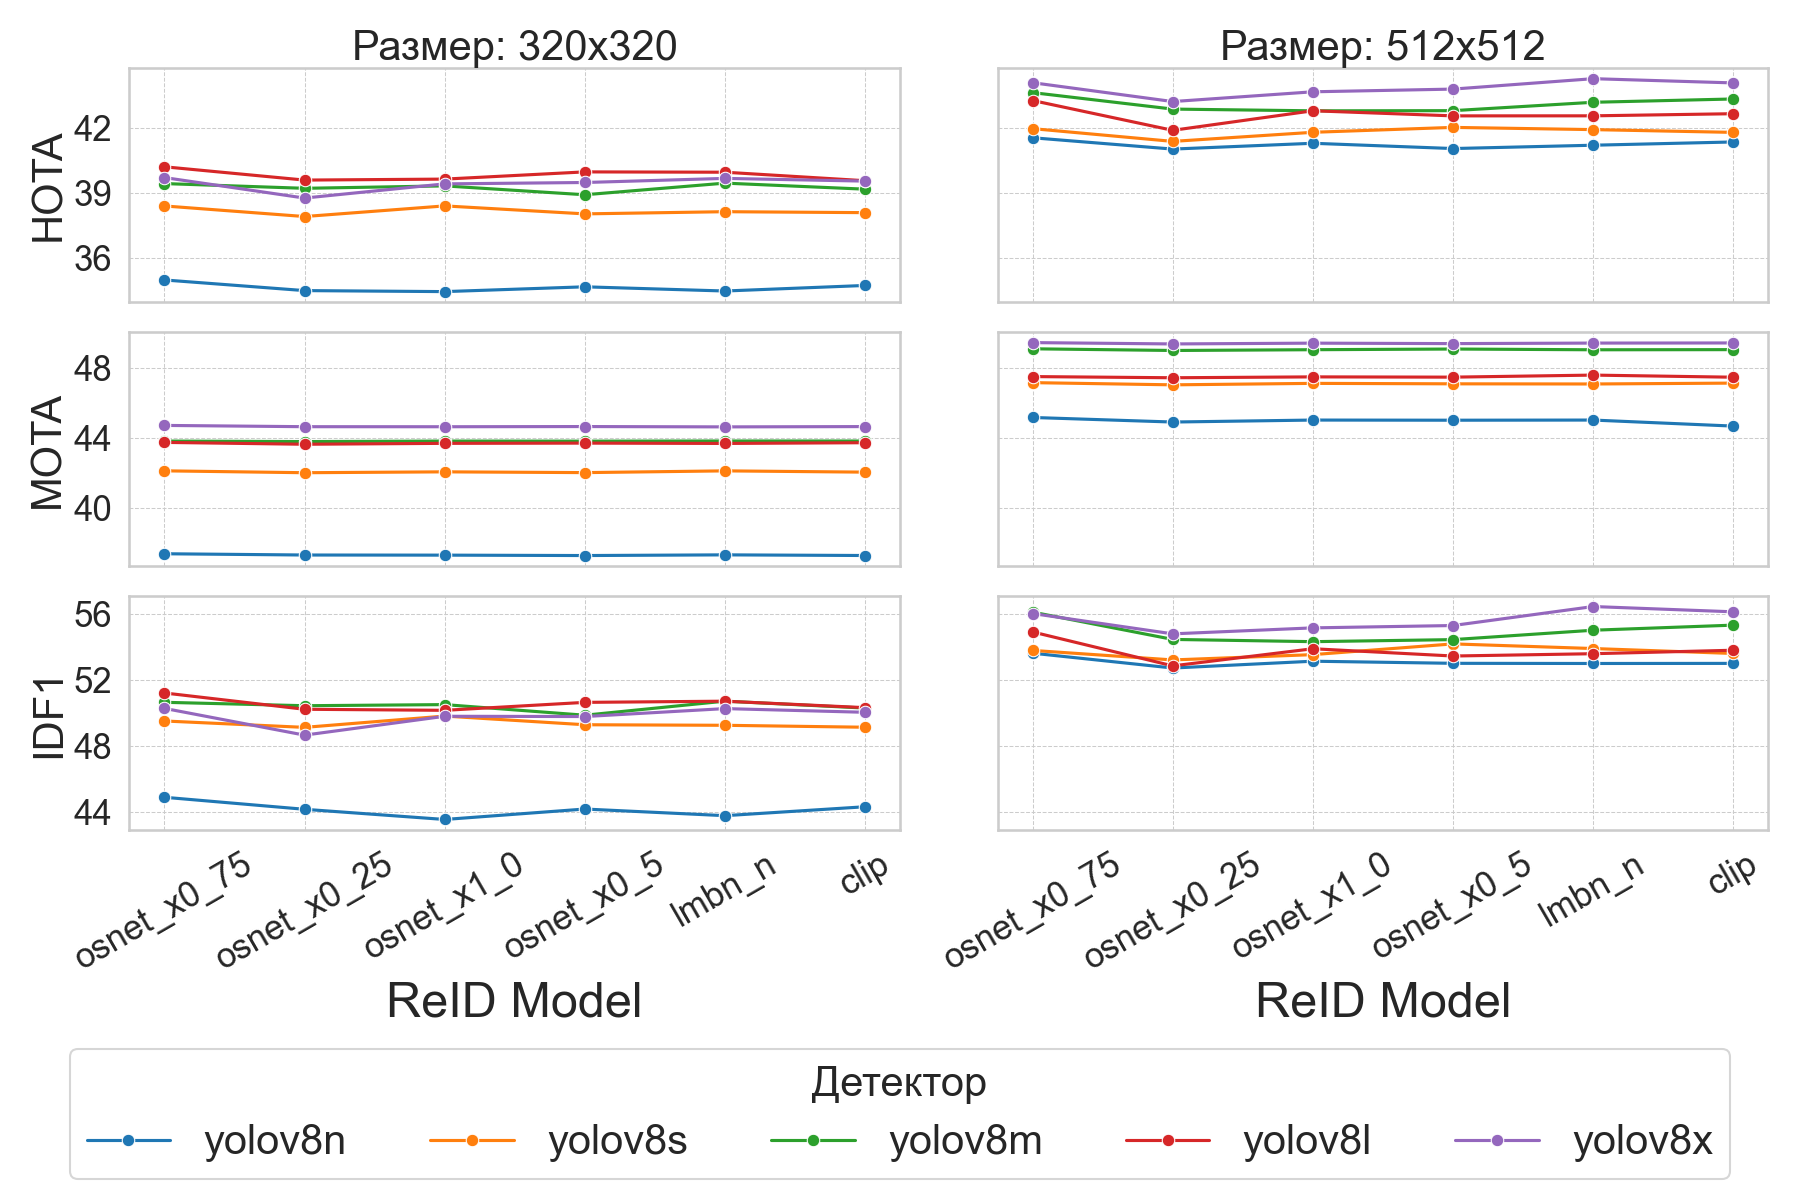
\includegraphics[width=1\textwidth]{plots/fps_vs_metric/ImprAssOC.png}
    \caption{График зависимости метрик HOTA, MOTA и IDF1 от частоты кадров видеоизображения для алгоритма ImprAssOC}
    \label{fig:fps_ImprAssOC}
\end{figure}
\FloatBarrier